\documentclass[a4paper,12pt]{article}
\usepackage{underscore}
\usepackage{ifthen}
\usepackage{amsmath}
\usepackage{graphicx}

\newcommand{\Tcg}{\textsc{Tcg}}
\newcommand{\code}[1]{\texttt{#1}}
\newcounter{premise}
\newcommand{\premise}[2]{
\ifthenelse{\equal{\arabic{premise}}{1}}{\\}{}%
    \setcounter{premise}{1}%
    #1\vdash#2%
}
\newcommand{\ifnotempty}[2]{\ifthenelse{\equal{#1}{}}{}{#2}}
\newcommand{\tcgrule}[5]{%
	\setcounter{premise}{0}%
$$%
    \ifnotempty{#1}{%
        \forall \left(#1\right)\;%
    }%
    \dfrac{%
	    \begin{array}[b]{l}%
	    #2%
            \end{array}%
    }{%
            #3%
    }%
    \;\ifnotempty{#4}{(\mathtt{#4}\ifnotempty{#5}{[\mathbf{#5}]})}%
$$%
}

\title{A Generator for Type Checkers\\ \small{A Ph.D. thesis by Holger Gast, 2004}}
\author{Andrey Breslav}

\begin{document}

\maketitle

\section{Introduction}

Tools for generating parsers for different types of context-free grammars have been available for decades. They serve for automating the routine task of developing a parser and make it less error-prone by working with high-level specifications, which are (in most cases, partially) declarative and checkable for consistence.

However, a context-free syntax does not capture all the features of a programming language. There remains the ``non-context-free syntax'' or ``static semantics'', which is checked by hand-written code. But one is unlikely to say that the type theory is underdeveloped compared to automata theory, thus we should expect availability of type-checker generators as well as parser generators. And these tools might be a big advantage for implementing non-context-free static checks.

This report is based on a Ph.D. thesis by H. Gast ``A Generator for Type Checkers'' \cite{Tcg}. Chapter 5 of the thesis examines the related work in detail, and we will not go into it here. The only thing we have to mention is that there were attempts to create such tools before, but most of them suffer from being more of domain-specific \emph{programming} languages than \emph{declarative} specification languages. The \textsc{Type Check Generator} (\Tcg{}) tool described in the thesis makes a significant advance towards the declarative style.



\section{Approach Overview}

We use types in programming languages to enforce certain properties of our programs at compile time. Types themselves (provided as annotation or inferred) can be thought of as statements about those properties, which the compiler (to be precise --- the type-checker subsystem of the compiler) proves in some way.

In \Tcg{} the type checking process is modeled as a search for explicit proofs of statements associated with an Abstract Syntax Tree (AST) of a program. The proofs are built with respect to inference rules specified by the user; in fact, the rules form the core part of a declarative specification of a type system in \Tcg{}. This approach is, of course, related to the Curry-Howard correspondence, but only in a broad sense: \Tcg{} builds proofs using the AST structure but not strictly according to it. 

A language of types used in \Tcg{} is limited only by very general requirements like having most general unifiers. Strictly speaking, we cannot always identify a type within a \Tcg{} statement, since a \emph{typing relation} ($e : t$) does not have to be present in it. And where present, types may have almost arbitrarily complicated structure. This structure, as well as the structure of proofs is described by \emph{typing rules} (specified by a user) which are basically inference rules of a proof system. 

Proofs are constructed by a procedure based on a depth-first backtracking search, which is basically a backwards reasoning facilitated by a sound set of operations over proofs which the user may trigger by referring to them in the typing rules (the proof structure along with the operations are formally described in Chapter 2 of \cite{Tcg}).

Beside the typing rules themselves, a \Tcg{} specification describes
\begin{itemize}
	\item context-free syntax;
	\item abstract syntax tree (AST) construction;
	\item pretty-printing rules.
\end{itemize}
At generation time (Figure 1) the translator produces a parser and an initial context for the proof search.

\begin{figure}[htp]
\centering
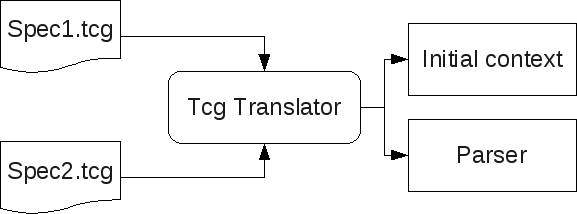
\includegraphics[width=.7\textwidth]{generator.png}
\caption{The \Tcg{} Generator}
\end{figure}

At runtime (Figure 2) the parser builds an AST and collects associated goals to be proven. Then it runs an ``interpreter'' which searches for proofs of the collected goals.

\begin{figure}[htp]
\centering
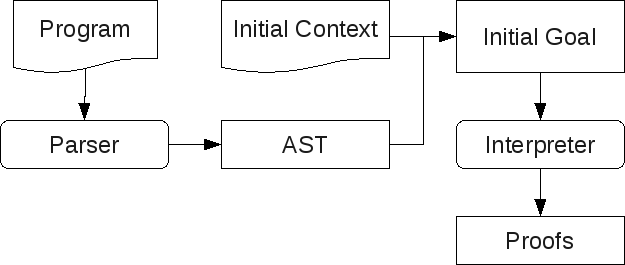
\includegraphics[width=.7\textwidth]{runtime.png}
\caption{The \Tcg{} Type Checker at Run Time}
\end{figure}

In this report we mainly illustrate the usage of \Tcg{} by giving examples of typing rules (aiming at implementing a type checker for the \textsc{MiniML} language \cite{MiniML}).
Since \Tcg{} rules include proof search instructions, the same set of examples will illustrate the main techniques used to direct the proof construction. Formal definitions of the rule language are given in Chapter 3 of \cite{Tcg}.


\section{\Tcg{} In Action}

Context-free syntax is described by YACC-style productions each grammar must have a start symbol called \code{file}. Productions may be annotated with AST building instructions (after \code{-->} sign) or a block of code to be executed after the production has been matched (in \code{\{!} \ldots{} \code{!\}} brackets). The \code{file} symbol is responsible for running type analysis, which is usually done by invoking the \code{run} command:

\begin{verbatim}
file: top_wrap EOF {! run ~save: 
                      [ (input.base^".rls",
                          [ ("define", "save_defined") ]) ] $1 
                   !}
\end{verbatim}

The arguments passed to the \code{run} command deal with saving results and are irrelevant for our discussion.

The rest of this section follows the logic and structure of the Chapter 4 of the original work \cite{Tcg}, explaining the formalism and other aspects of \Tcg{} by giving examples which start with the classical simply-typed $\lambda$-calculus and go through all the features of the \textsc{MiniML} language \cite{MiniML}.

\subsection{Symply-Typed $\lambda$-Calculus}

The context-free syntax of the simply-typed $\lambda$-calculus is described by the following rules (we omit lexical definitions and documenting annotations):

\begin{verbatim}
top_wrap: tops        --> tops($1)

tops: top             --> $1 :: []
    | top ";;" tops   --> $1 :: $3

top: exp              --> $1

exp: ID               --> id[$1]
   | exp exp          --> apply($1,$2)
   | "\\" ID "." exp  --> lambda(id[$2],$4)
   | "(" exp ")"      --> $2
\end{verbatim}

The first three rules describe a sentence as a list of expressions (\code{exp}) separated by double-semicolons (\code{";;"}). The last rule describes a $\lambda$-expression in a usual way: as a variable, application, abstraction or bracketed expression. As mentioned before, instructions after the \code{-->} symbols serve for AST-construction; there are several types of such instructions:
\begin{itemize}
 \item item references of the form \code{\$<number>} --- reference items on the left-hand side;
 \item node constructors of the form \code{<node_type>(<children>)};
 \item list constructors of the form \code{head::tail}, where \code{[]} denotes the empty list;
 \item opaque term constructors of the form \code{<class>[<value>]} -- these will be explained later.
\end{itemize}

For example, a textual representation of the expression 
$$(\lambda f.\lambda x. f\; x)\; g\; y$$
will be \\
``\code{(\textbackslash f.\textbackslash x.f x) g x}'', \\
and an AST constructed from it is%
\begin{verbatim}
tops(
    apply(
        apply(
            lambda(id[f], 
                lambda(id[x], 
                    apply(id[f], id[x]))),
            g),
        x)
    ::[]
)
\end{verbatim}

A \emph{typing judgement} in \Tcg{} is a pair 
$$term : type$$
where $term$ is an AST subtree and $type$ is a term which structure is defined by typing rules. The typing rules are used by \Tcg{} to construct proofs of typing judgements, which are basically trees where the proven judgement is a root and all the edges are \emph{properly} labeled with rules (what ``properly'' means will be explained later). 

A generic typing rule consists of a set of universally quantified \emph{variables}, a list of \emph{premises}, a \emph{conclusion} and a list of \emph{parameters}. In \Tcg{}'s concrete syntax it is written like this:
\begin{verbatim}
rule apply
  forall(f,e,s,t)
    apply(f,e) : t
  if f : fun(s,t)
  and e : s
\end{verbatim}

In this example, \code{f}, \code{e}, \code{s} and \code{t} are the quantified variables, \code{apply(f,e)} is the conclusion, \code{f:fun(s,t)} and \code{e:s} are the premises. In the more familiar notation of inference rules it can be written like this:
\tcgrule{f, e, s, t}{
    \Gamma \vdash f : s \rightarrow t
    \hspace{20pt}
    \Gamma \vdash e : s
}{\Gamma \vdash f\; e : t}{apply}{}

This rule expresses the typing for an application. To construct a proof for a judgement $f\;e : t$ we have to build a tree, where this judgement will be the root node and its children will be obtained by \emph{application} of this rule. So the root node will have two children having the forms of the premises, where $f$, $e$ and $t$ are already known (they appear in the initial judgement) and $s$ must be inferred. Each node in the tree is marked with the rule applied at this node, in our case the root node will be marked with \code{apply} rule. To complete the proof we must construct subtrees proving the children, so that leaves of the tree will be marked with application of rules which have no premises. This example provides a rough intuition about proof structure, we will improve it further (for formal definitions see Chapter 2 of the original thesis).

We have written $\Gamma$ in the example above to provide the most familiar notation, but in \Tcg{} the context is ``global'' for the rule application and is being modified each time a rule is applied (the modified version is relevant to the subtree of the vertex marked with the applied rule). This is motivated by the backward style of reasoning adopted by \Tcg{}: when we apply a rule, we create new vertices in the proof tree and change our knowledge about currently available typing information. These changes are expressed by \emph{context modifiers} which are written in the premises instead of context variables like $\Gamma$. For example, here is the rule for $\lambda$-abstraction:
\begin{verbatim}
rule lambda
  forall(x,e,s,t)
    lambda(x,e) : fun(s,t)
  if e : t
    under -( :.1.= x) + [ x : s ]
\end{verbatim}
Here is the tree-like form of this rule:
\tcgrule{x, e, s, t}{
    \premise{-( :_1 = x), +[ x : s ]}{e : t}
}{\lambda x. e : fun(s,t)}{lambda}{}
The context modifiers here are \code{-(:.1. = x)} and \code{+[ x : s ]}. The first one removes rules assigning a type to $x$ from the context of the conclusion, it consists of two parts: a minus sign, which denotes removal and a \emph{selector}
$$:_1 = x$$
which is basically a pattern meaning that the top function symbol in terms we are going to delete is a colon and its first argument is $x$. Another context modifier in this example adds a new typing fact, $x : s$.

The context modifiers are applied to the context available a the root of the subtree, so they are relative to the context of the conclusion, that is why we do not write anything denoting context under the like.

The rule \code{apply} mentioned above has no context modifiers, thus in tree-like form it is written as follows:
\tcgrule{f, e, s, t}{
    \premise{}{f : s \rightarrow t}
    \premise{}{e : s}
}{f e : t}{apply}{}

The third rule for simply-typed $\lambda$-calculus will be the following:
\tcgrule{es, ts}{
\premise{}{\mathtt{[branch]}\; es : ts \; \mathbf{export} * \ldots}
}{tops(es)}{tops}{}
Note that the conclusion here is not a typing judgement; there is no problem: we are basically proving a theorem and our language is not limited to a single predicate ``:''. The premise contains a \code{[branch]} modifier which denotes that it must be looked for by a independent sub-search procedure; the ellipsis \code{...} is a shorthand denoting list iteration: in our AST structure \code{tops} contains a list of children, so the \code{es} variable will iterate through it item-by-item.

The final spet is to construct an initial set of rules, which are available at the beinning of the proof search.  We put all our rules there:
\begin{verbatim}
environment apply,lambda,tops
\end{verbatim}

\subsection{Introducing Constants}

Assume we want to have integer or boolean literals in our language. These will by represented by corresponding tokens: \code{INT}, \code{``true''} and \code{``false''}. AST productions for these will be the following:
\begin{verbatim}
    INT     --> int[$1]
  | "false" --> bool["false"]
  | "true"  --> bool["true"]
\end{verbatim}

As we have seen before, here \emph{opaque} terms, e.g. \code{int[\$1]}, are constructed instead of normal AST nodes, these terms are opaque for the type checker: it can not look inside them, and can only consider their classes (\code{int} and \code{bool} in our case), but the values can be extracted for output (e.g., for error reporting).

Typing rules for such constants will be of the following form:
\tcgrule{i}{}{\mathtt{int[}i\mathtt{]}:\mathtt{int}}{int\_const}{}

We can declare ``primitive'' or ``built-in'' operations in the same manner:
\tcgrule{}{}{add : int \rightarrow int \rightarrow int}{add\_function}{}

And likewise are conditional expressions:
\tcgrule{e_1,e_2,e_3,t}{
\premise{}{e_1 : bool}
\premise{}{e_2 : t}
\premise{}{e_3 : t}
}{\mathbf{if}\; e_1\; \mathbf{then}\; e_2\; \mathbf{else}\; e_3\; \mathbf{endif} : t}{if\_expr}{}

\subsection{Bindings}

For the monomorphic version of let expression (\code{let x = e in e'}) it is sufficient to treat it as $\lambda$ abstraction applied to the bound term: $(\lambda x.e')\;e$. Thus we can write down the following rule:
\tcgrule{x,e,e',s,t}{
\premise{}{e' : s}
\premise{-(:_1 = x), +[x : s]}{e : t}
}{\mathbf{let}\;x = e'\;\mathbf{in}\;e : t}{mono\_let}{}

In case of polymorphism, which means that $x$ may be typed with $\forall \widetilde{\alpha}.s$, this approach will not work directly, since we need to quantify all the \emph{inner variables} of the type scheme $s$, which are the variable which appear freely in the proof of $e' : s$ and do not appear in other parts of the proof tree. The operators presented by now do not allow to do this, so \Tcg{} introduces more tools which are expressive enough to cover it (and much more): \emph{rule extraction} and \emph{forward application}. To illustrate these techniques, we will first reformulate the above rule \code{mono\_let} and then extend it to a polymorphic version.

Rule extraction basically just takes a (possibly incomplete) subproof and turns it into a new rule: the root of the subproof becomes a conclusion, and the leafs become premises. If the subproof was complete, then there will be no premises in the rule (all the premises will be empty). This operation corresponds to the idea of memorizing subproofs as lemmata and re-using them in different parts of the proof. Thus we are going to extract a proof of $e' : s$ and then use it in the proof for the second premise (and later for the proof of $\forall x : \widetilde{\alpha}.s$).

By now we can easily prove $e' : s$, but what we need for the second premise is $x : s$. This is where forward application comes into the stage: it allows to combine two rules into one if the premise of the second rule unify with the conclusion of the first one.
$$
\left.\begin{array}{r}
	\tcgrule{}{\ldots}{e' : s}{}{}\\
	+\hspace{14pt}\\
	\tcgrule{e,t}{e : t}{x : t}{}{}
\end{array}
\right\}
\Rightarrow 
\begin{array}{l}
	\tcgrule{}{\ldots}{x : t}{}{}
\end{array}
$$
This operation easily generalizes to more than one premise of the second rule.

Now we can reformulate \code{mono_let} in this manner: in the context modifier for the second premise, we will extract the proof of the first premise and apply the forward reasoning.
\tcgrule{x,e,e',s,t}{
    \premise{}{e' : s}
    \premise{-(:_1 = x), +[\mathtt{let\_binding}[x]](\langle 1 \rangle)}{e : t}
}{\mathbf{let}\;x = e'\;\mathbf{in}\;e : t}{let\_subproof}{}

The auxiliary rule \code{let_binding} looks like this:
\tcgrule{e,t}{\premise{}{e : t}}{\mathbf{y} : t}{let\_binding}{y}

Let us explain the new pieces of notation now. First, we have a \emph{rule reference} in the context modifier of the first premise:
$$\mathtt{let\_binding}[x]$$
this simply adds the rule \code{let_binding} to the context, passing $x$ to it as an argument. As you can see, the rule has a formal parameter $\mathbf{y}$; this parameter must be instantiated with a term upon the rule application; in our case it is instantiated with the term $x$.

The rule reference is followed by a forward application:
$$[\mathtt{let\_binding}[x]](\langle 1 \rangle)$$
this notation means ``extract the proof of the first premise and apply forward reasoning to it an the rule $\mathtt{let\_binding}[x]$''. The generic syntax for this operation will be
$$rule\_expression(rule\_expressions)$$
where each rule expression may be 
\begin{itemize}
	\item an inline rule (e.g., $x : s$), 
	\item a reference (e.g., $\mathtt{let\_binding}[x]$), 
	\item a rule extracted from the subproof of the premise number $i$ (e.g., $\langle 1 \rangle$, the premise must stay to the left of the current premise),
	\item the \textbf{environment} which refers to all the rules present in the context.
\end{itemize}

Now we proceed to the polymorphic version of \textbf{let}. To complete the definition, we change \code{let_subproof} only slightly:
\tcgrule{x,e,e',s,t}{
    \premise{}{e' : s}
    \premise{-(:_1 = x), +[\mathtt{let\_binding}[x]](\langle 1 : [\forall] \rangle)}{e : t}
}{\mathbf{let}\;x = e'\;\mathbf{in}\;e : t}{let\_poly}{}

Here $\langle 1 : [\forall] \rangle$ stands for ``extract the subproof of the first premise and quantify its inner variables universally''. These will be exactly $\widetilde{\alpha}$ --- the variables quantified in the type scheme $\forall \widetilde{\alpha}.s$. Note that the type scheme itself does not appear in the rule: we do not need to enrich our predicate language with universal quantification since it is successfully handled by the meta-theory. Why is the meta-theory designed in such a way that is serves exactly this purpose? The author of the original work gives a detailed explanation in the Section 4.1.3.3, to put it shortly: quantifying the free variables is a natural operation which makes a rule usable, and inner variables are the maximal set of variables which can be quantified without affecting soundness.

\subsection{Recursion}

To define non-trivial functions with \textbf{let}, we need recursion, which is not yet supported by our rule. To support it we can just add a context modifier to the first premise:
\tcgrule{x,e,e',s,t}{
    \premise{+[x : s]}{e' : s}
    \premise{-(:_1 = x), +[\mathtt{let\_binding}[x]](\langle 1 : [\forall] \rangle)}{e : t}
}{\mathbf{let}\;x = e'\;\mathbf{in}\;e : t}{let\_poly}{}

By doing this we have added the assumption $x : s$ to the proof for $e' : s$, and since $x$ is being bound to $e'$ this indeed enables recursion. 

By now we can handle all the basic functionality available in a functional language. In further subsections we illustrate more sophisticated features of \Tcg{} by extending the capabilities of the language with more convenient mechanisms like multi-binding \code{let} and mutual recursion.

\subsection{Parallel bindings}

To make our language more practical, let us introduce \code{let} expressions binding many variables at the same time. The syntax will be the following:

\begin{verbatim}
exp: "let" bind_group "in" exp    --> let($2,$4)

bind_group: bind                  --> $1 :: []
          | bind "and" bind_group --> $1 :: $3

bind: ID "=" exp                  --> bind(id[$1],$3)
\end{verbatim}

In the AST a bind group is represented by a \emph{list} of bindings. Now we cannot write a rule of the from 
\tcgrule{}{
    \premise{}{typings\; of\; bindings}
    \premise{+[\mathtt{let\_binding}[x]](\langle bindings : [\forall] \rangle)}{e : t}
}{\mathbf{let}\;bindings\;\mathbf{in}\;e : t}{}{}

because \emph{typings of bindings} is not a single premise, but a list of variable length. Instead, we can process the list by usual recursion:
%
$$\begin{array}{cc}
\tcgrule{}{
    {\vdash head}
    \hspace{15pt}
    {\vdash \mathtt{bind\_group}(tail)}
}{\mathtt{bind\_group}(head\;\mbox{\tt ::}\;tail)}{}{}
&
\tcgrule{}{}{\mathtt{bind\_group}(\mbox{\tt []})}{}{}
\end{array}$$

Then, the \code{let} rule will look like this:
\tcgrule{bs,e,t}{
\premise{}{\mathtt{bind\_group}(bs)}
    \premise{+[???](\langle ??? : [\forall] \rangle)}{e : t}
}{\mathbf{let}\;bs\;\mathbf{in}\;e : t}{}{}

The question marks indicate that by now we do not know what to extract from the premise and what to compose it with. Indeed, what we did in the previous example was extracting a subproof which ended with a typing judgement $e' : s$, but here the premise is not a typing judgement, judgements are ``hidden'' in its proof:
%
\tcgrule{}{
\begin{array}{cl}
	e'_1 : s_1\;\dots\;e'_n : s_n&\\
	\vdots&\\
	\vdash {\mathtt{bind\_group}(bs)}&\;\;
    \premise{\ldots(\langle proofs\; for\; e_1\ldots e_n : [\forall] \rangle)}{e : t}
\end{array}
}{\mathbf{let}\;bs\;\mathbf{in}\;e : t}{}{}

\Tcg{} provides a generalized for of rule extraction which is useful here: the rules may be marked with ``\textbf{export} \emph{label}'', the label will be put on the proof tree nodes; the extracting operator may be directed to extract not the whole tree but only the subtrees marked with a certain label. Not all the label in a proof tree are visible from its root, but only those which were \emph{propagated} up the tree. If a node in the tree is marked with a special label ``$*$'', it propagates labels of all the child nodes up. To be able to extract all the needed typing judgements from the proof of $\mathtt{bind\_group}(bs)$, we can do the following:
$$\begin{array}{cc}
\tcgrule{}{
    {\vdash head\;\mathbf{export}\; \mathtt{bind}}
    \hspace{15pt}
    {\vdash {bind\_group}(tail)\;\mathbf{export}\;*}
}{{bind\_group}(head\;\mbox{\tt ::}\;tail)}{}{}
&
\tcgrule{}{}{{bind\_group}(\mbox{\tt []})}{}{}
\end{array}$$

By doing this, we label every typing judgement from $bs$ and propagate these labels up the tree when doing a recursive call. This situation is rather common, so \Tcg{} provides a shorthand for it: to handle lists we can use ellipsis (\ldots) at the premise, this will tell the system to generate the two rules given above. Now we can complete the initial rule:
\tcgrule{bs,ts,e,t}{
\premise{}{bs : ts \;\mathbf{export}\; \mathtt{bind} \; \ldots}
\premise{+[\mathtt{exp\_binding}](\langle 1 : \mathtt{bind} [\forall] \rangle)}{e : t}
}{\mathbf{let}\;bs\;\mathbf{in}\;e : t}{}{}

The extraction operator is now $\langle 1 : \mathtt{bind} [\forall] \rangle$, which will extract from the proof of the first premise all the subproofs labeled with \texttt{bind} and universally quantify the inner variables \emph{of the whole proof} of the first premise (this ``over-quantification'' is safe). Note that the variable $ts$ is free, so it will be quantified. The auxiliary rule \code{exp_binding} is the following:
\tcgrule{x,e,t}{\premise{}{x = e : t}}{x : t}{exp\_binding}{}

We also need a rule to be able to rove judgements of the form $x = e : t$. It is straightforward:
\tcgrule{x,e,t}{\premise{}{e : t}}{x = e : t}{binding}{}

\subsection{Mutual Recursion}

To typecheck a mutually recursive definition like this
\begin{verbatim}
  letrec even = \x. if (eq_int x) 0 then true else odd ((sub x) 1)
     and odd = \x. if (eq_int x) 0 then false else even ((sub x) 1)
  in even 5
\end{verbatim}
we need to choose fresh type variables $\alpha_1$ and $\alpha_2$ and assume $even : \alpha_1$ and $odd : \alpha_2$ before the right-hand sides of the bindings. This procedure is different from what we have seen by now in a way that it needs ``a lookahead'', in other words, we cannot look at every item in the program only once. To handle this, we write the following rules:
\tcgrule{bs,e,t,x}{
\premise{}{bind\_group(bs)\;\mathbf{export}*}
\premise{-(:_1 = x \rightarrow :_1 = x); +[\mathtt{exp\_binding}](\langle 1 : \mathtt{bind} [\forall] \rangle)}{}
\\{e : t}
}{\mathbf{letrec}\;bs\;\mathbf{in}\;e : t}{letrec}{}
%
\tcgrule{bs,ts,x}{
\premise{}{bs : ts \;\mathbf{export}\;\mathtt{fwd}\;\ldots}
\premise{-(:_1 = x \rightarrow :_1 = x); +[\mathtt{exp\_binding}](\langle 1 : \mathtt{fwd} \rangle)}{}
\\{bs : ts\;\mathbf{export}\;\mathtt{bind}\;\ldots}
}{{bind\_group}(bs)}{bind\_group}{}

The first premise of the rule \code{letrec} contains the most significant information: all the recursive definitions are checked there. The check itself is done by the \code{bind_group} rule, which iterates over the first premise, checks each element in $bs$ and marks the result with \code{fwd} label. These results will have the form $x = e : \alpha$ for a fresh $\alpha$ since $ts$ does not appear anywhere else in the rule, thus there is nothing to prove about such judgements, and we can make \Tcg{}'s life easier by marking them as \emph{solved goals} (done by putting ``!'' after the \code{fwd} label). The overall process precisely mimics what was discussed for the code example above: we take fresh type variables, assume typings for bound variables and check the expressions to the right of ``=''.

The context modifier $-(:_1 = x \rightarrow :_1 = x)$ is a \emph{guarded} one: it is triggered by adding a rule matching $:_1 = x$ (to the left of the arrow) is added, namely, it removes all the previously existing bindings for $x$ when a new binding is added.

\section{Conclusion}

We have illustrated the usage of \Tcg{} by developing a type system for the \textsc{MiniML} programming language, which supports mutually recursive polymorphic functions. While doing this we have used most features of the generator, so the reader has had a chance to overview the system. Our examples have shown that the specification language is purely declarative and rather concise.

The original paper \cite{Tcg} provides many interesting examples, which we did not cover, such as imperative languages, object-oriented languages and a language for stating generic algorithms with explicit requirements on their parameter types. These examples show that the approach works for large variety of type systems, not only functional languages with Hindley-Milner type inference. 

The original paper also provides comparison with other approaches to type system specification (Chapter 5), such as TYPOL, \textsc{TinkerType}, constraints solving and logical frameworks (\textsc{Isabelle}). These comparisons bring the evidence of \Tcg{} being, on the one hand, much less of a (logical) programming languages than previous solutions, on the other hand,  an fully specialized integrated framework as opposed to constraint solvers and logical frameworks. On the ``technical'' level the ability of subproof extraction is a distinguishing feature of \Tcg{}.

A major disadvantage which may prevent this approach from being used in practice might be the lack of comprehensible error reporting: when no proof is found (which means that the program is not correct), a type checker must complain with a helpful error message mentioning the reason of the problem; this aspect was not studied in the \cite{Tcg}.

\begin{thebibliography}{99}
	\bibitem[G04]{Tcg} H. Gast, A Generator for Type Checkers, \textit{Ph.D. Thesis}, Eberhard-Karls-Universit\"at T\"ubingen, 2004.
	\bibitem[CDDK86]{MiniML} D. Cl\'{e}ment, J. Despeyroux, T. Despeyroux, and G. Kahn. A Simple Applicative Language: Mini-ML. \textit{In Proceedings of the 1986 ACM Conference on LISP and Functional Programming}, pages 13–26, Cambridge, Massachusetts, USA, August 1986. ACM.
\end{thebibliography}
\end{document}

